We present and analyze resulting routes for three agents:
Alice, Bob, and Cal.
This is assuming no auxiliary metric datasets uploaded
so that the agents focus on time and fare.
Fixing their where and when information, we show how
agents' different constraints and preferences affect
their optimal routes computed by our planner.
Their where and when are set so that they all plan to
travel from San Jose International Airport (SJC) in
San Jose, to Pier 39 in San Francisco.
Note that the natural constraint $\psi$ in \eqtref{ex} 
is implicitly imposed on all cases.

Agent Alice has only one constraint that she does not 
have a car; thus, driving to her is never available during this trip.
Per her preferences, Alice provides her thoughts as earlier;
that is, public transportation is preferred to taxi, which is
better than biking, preferred to walking.
What's more, she decides that she would sacrifice thirty dollars
to save one hour during the trip.

The resulting route for Alice is included in \figref{alice}.
The solution takes 2 hours 7 minutes and 18 dollars 94 cents.
It is optimal in the sense the combined value of time
and fare is minimal among all paths from SJC to Pier 39.

\begin{figure}[!ht]
  \centering
    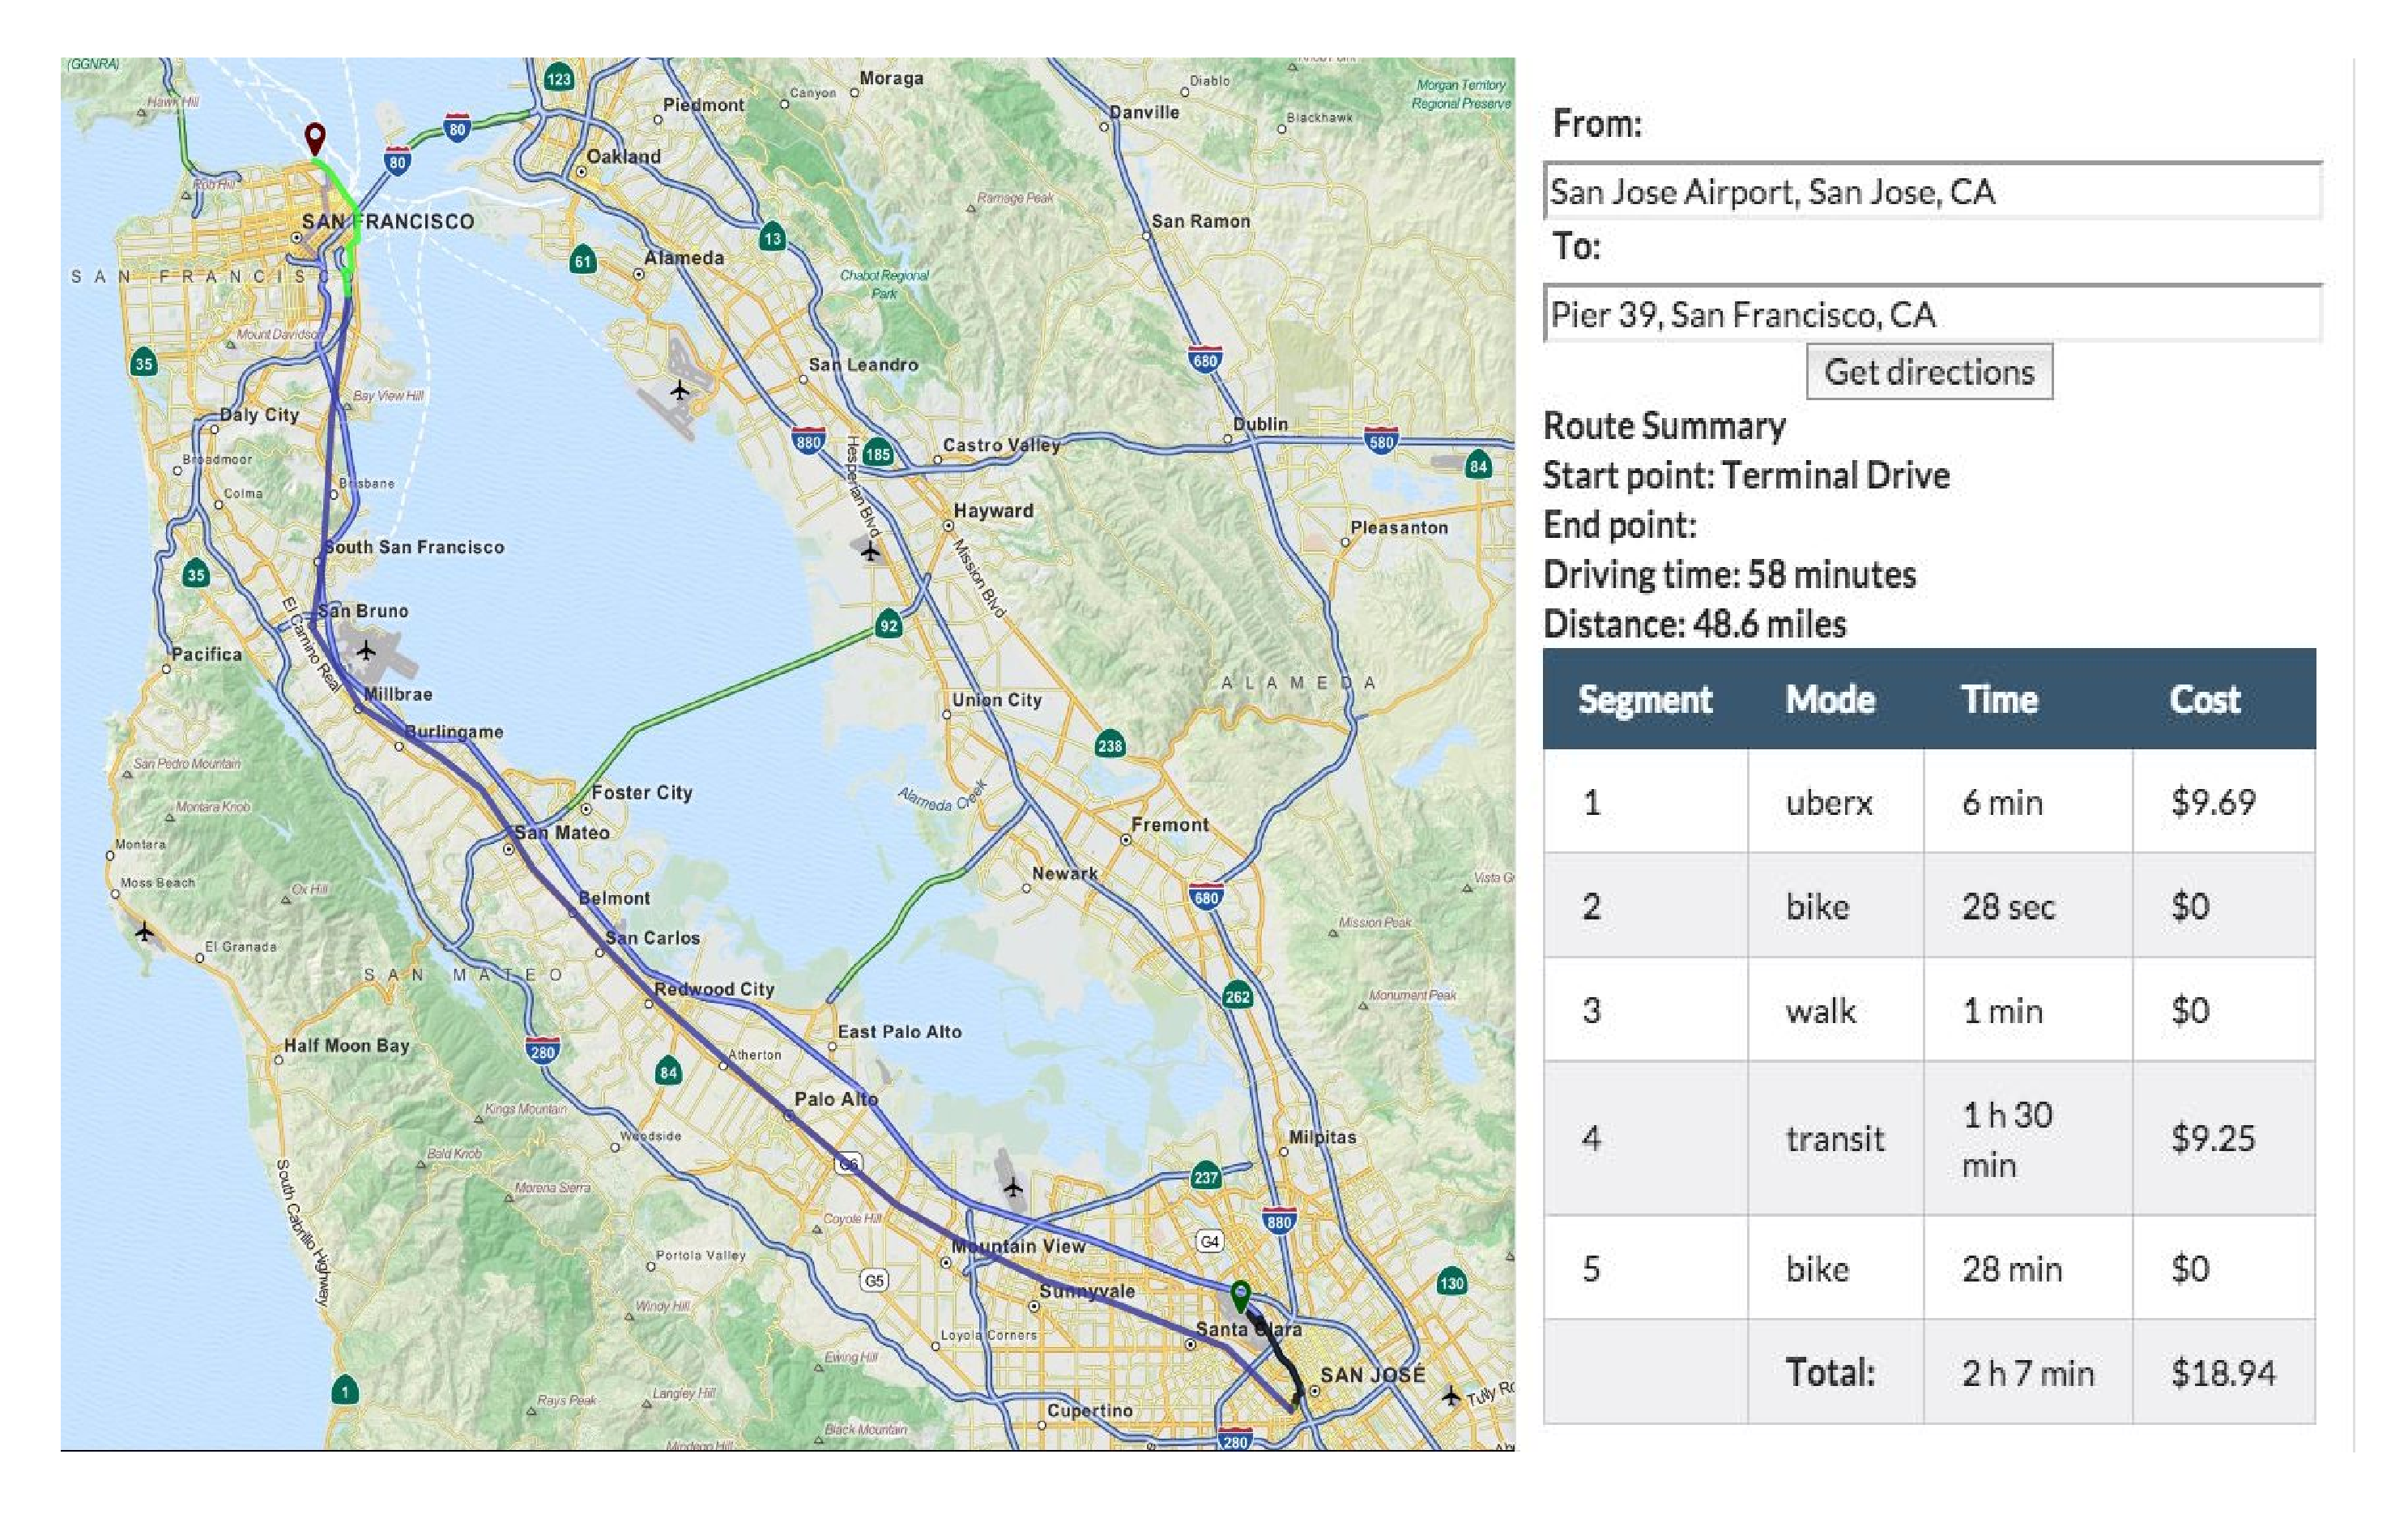
\includegraphics[width=0.5\textwidth]{figs/result_Alice.pdf}
  \caption{Resulting route for Alice\label{fig:alice}}
\end{figure}

Like Alice, Bob is constrained that he will not drive a car in his travel,
and his dollar per hour is thirty.
Moreover, Bob makes his mind to have some workout with his bike and
dictates that he will bike for between one and two hours.
He expresses his preferences: biking and public transit are the most
preferred, next is taxi, and the least preferred is walking.
Similarly, he has done so by answering the aforementioned elicitation questions.

The result for Bob is depicted in \figref{bob}.
It spans 2 hours 57 minutes in time with the fare of 29 dollars 17 cents.
It is so, seemingly worse than what Alice achieved, only because Bob has
the constraint that he will for sure bike for one to two hours, and
the preferences that put biking the most satisfying mode.

\begin{figure}[!ht]
  \centering
    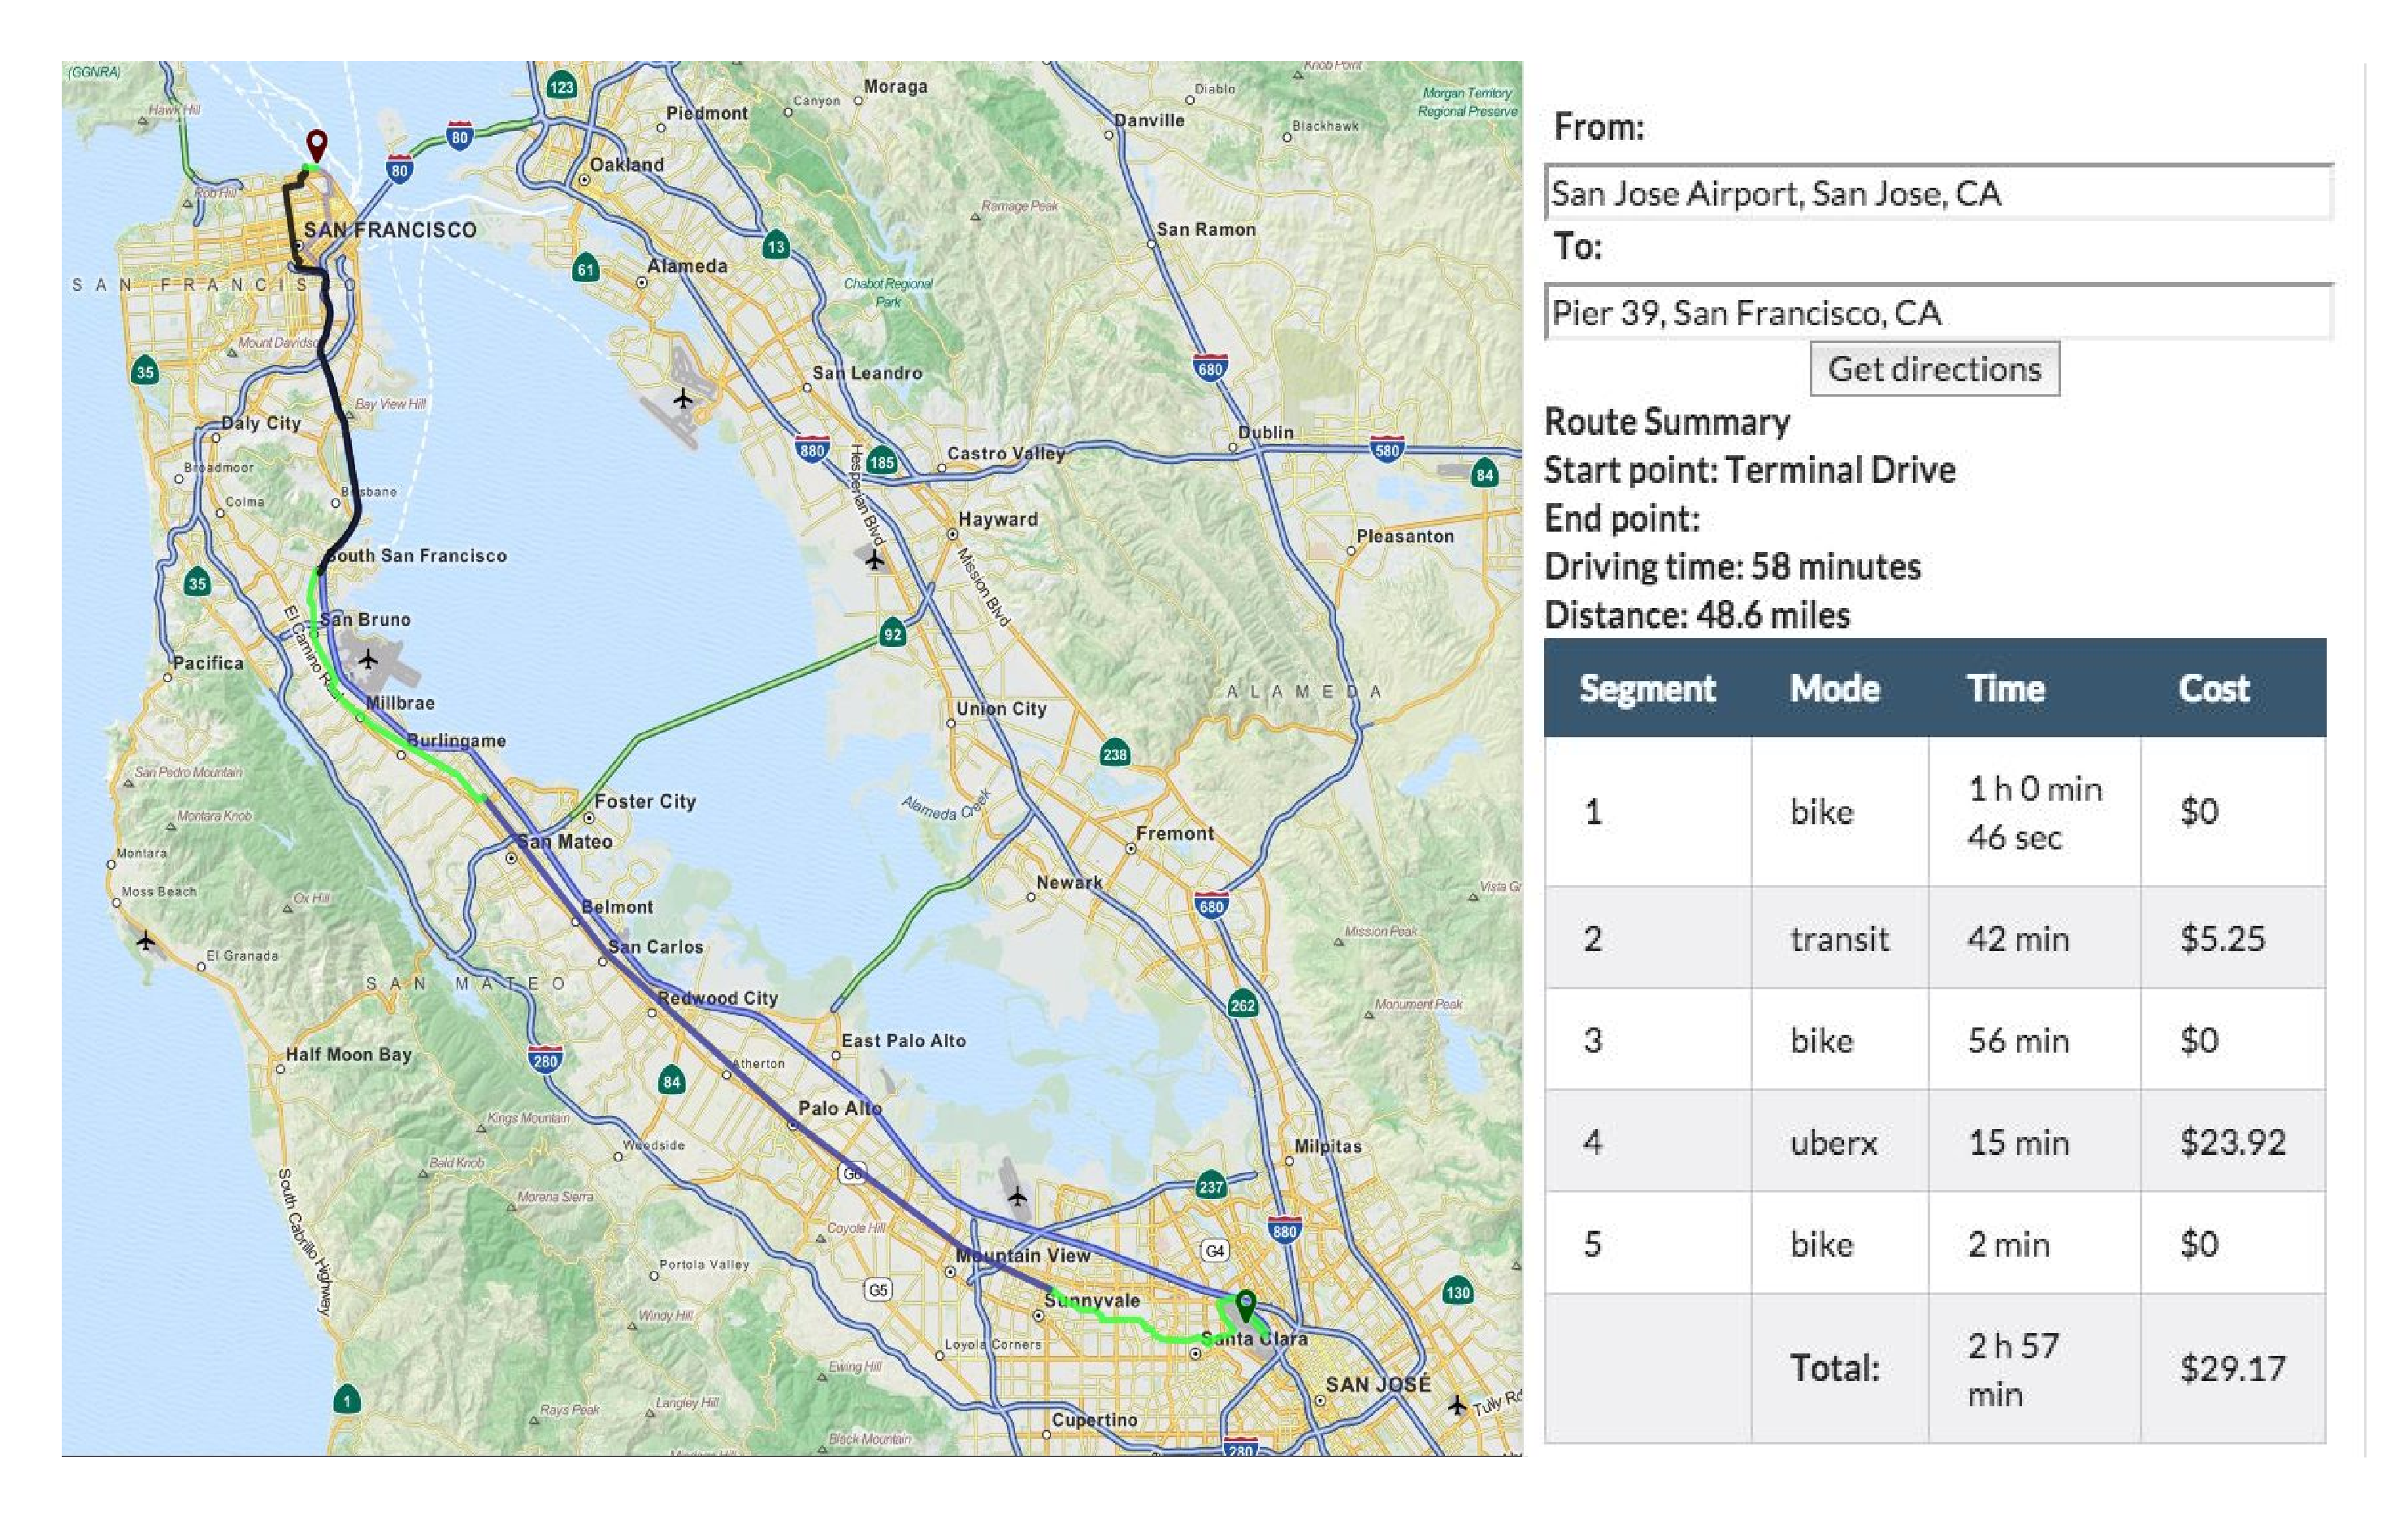
\includegraphics[width=0.5\textwidth]{figs/result_Bob.pdf}
  \caption{Resulting route for Bob\label{fig:bob}}
\end{figure}


Agent Cal will also not use a car in the trip.
He affirms that time is greatly valuable and one hour is measured
to 500 dollars, although his budget is restricted to 50.
Cal's preferences are that the most preferred are public transit
and taxi, and the next preferred are walking and biking that
are equivalent.

Refer to \figref{cal} for the optimal path for Cal.
This route, stretching 1 hour 48 minutes, is the most time-saving one 
compared with the previous two, at the price of 49 dollars 91 cents.
This is due to the constraint that Cal can spend up to 50 dollars,
as well as his preferences and vale of time being high.

\begin{figure}[!ht]
  \centering
    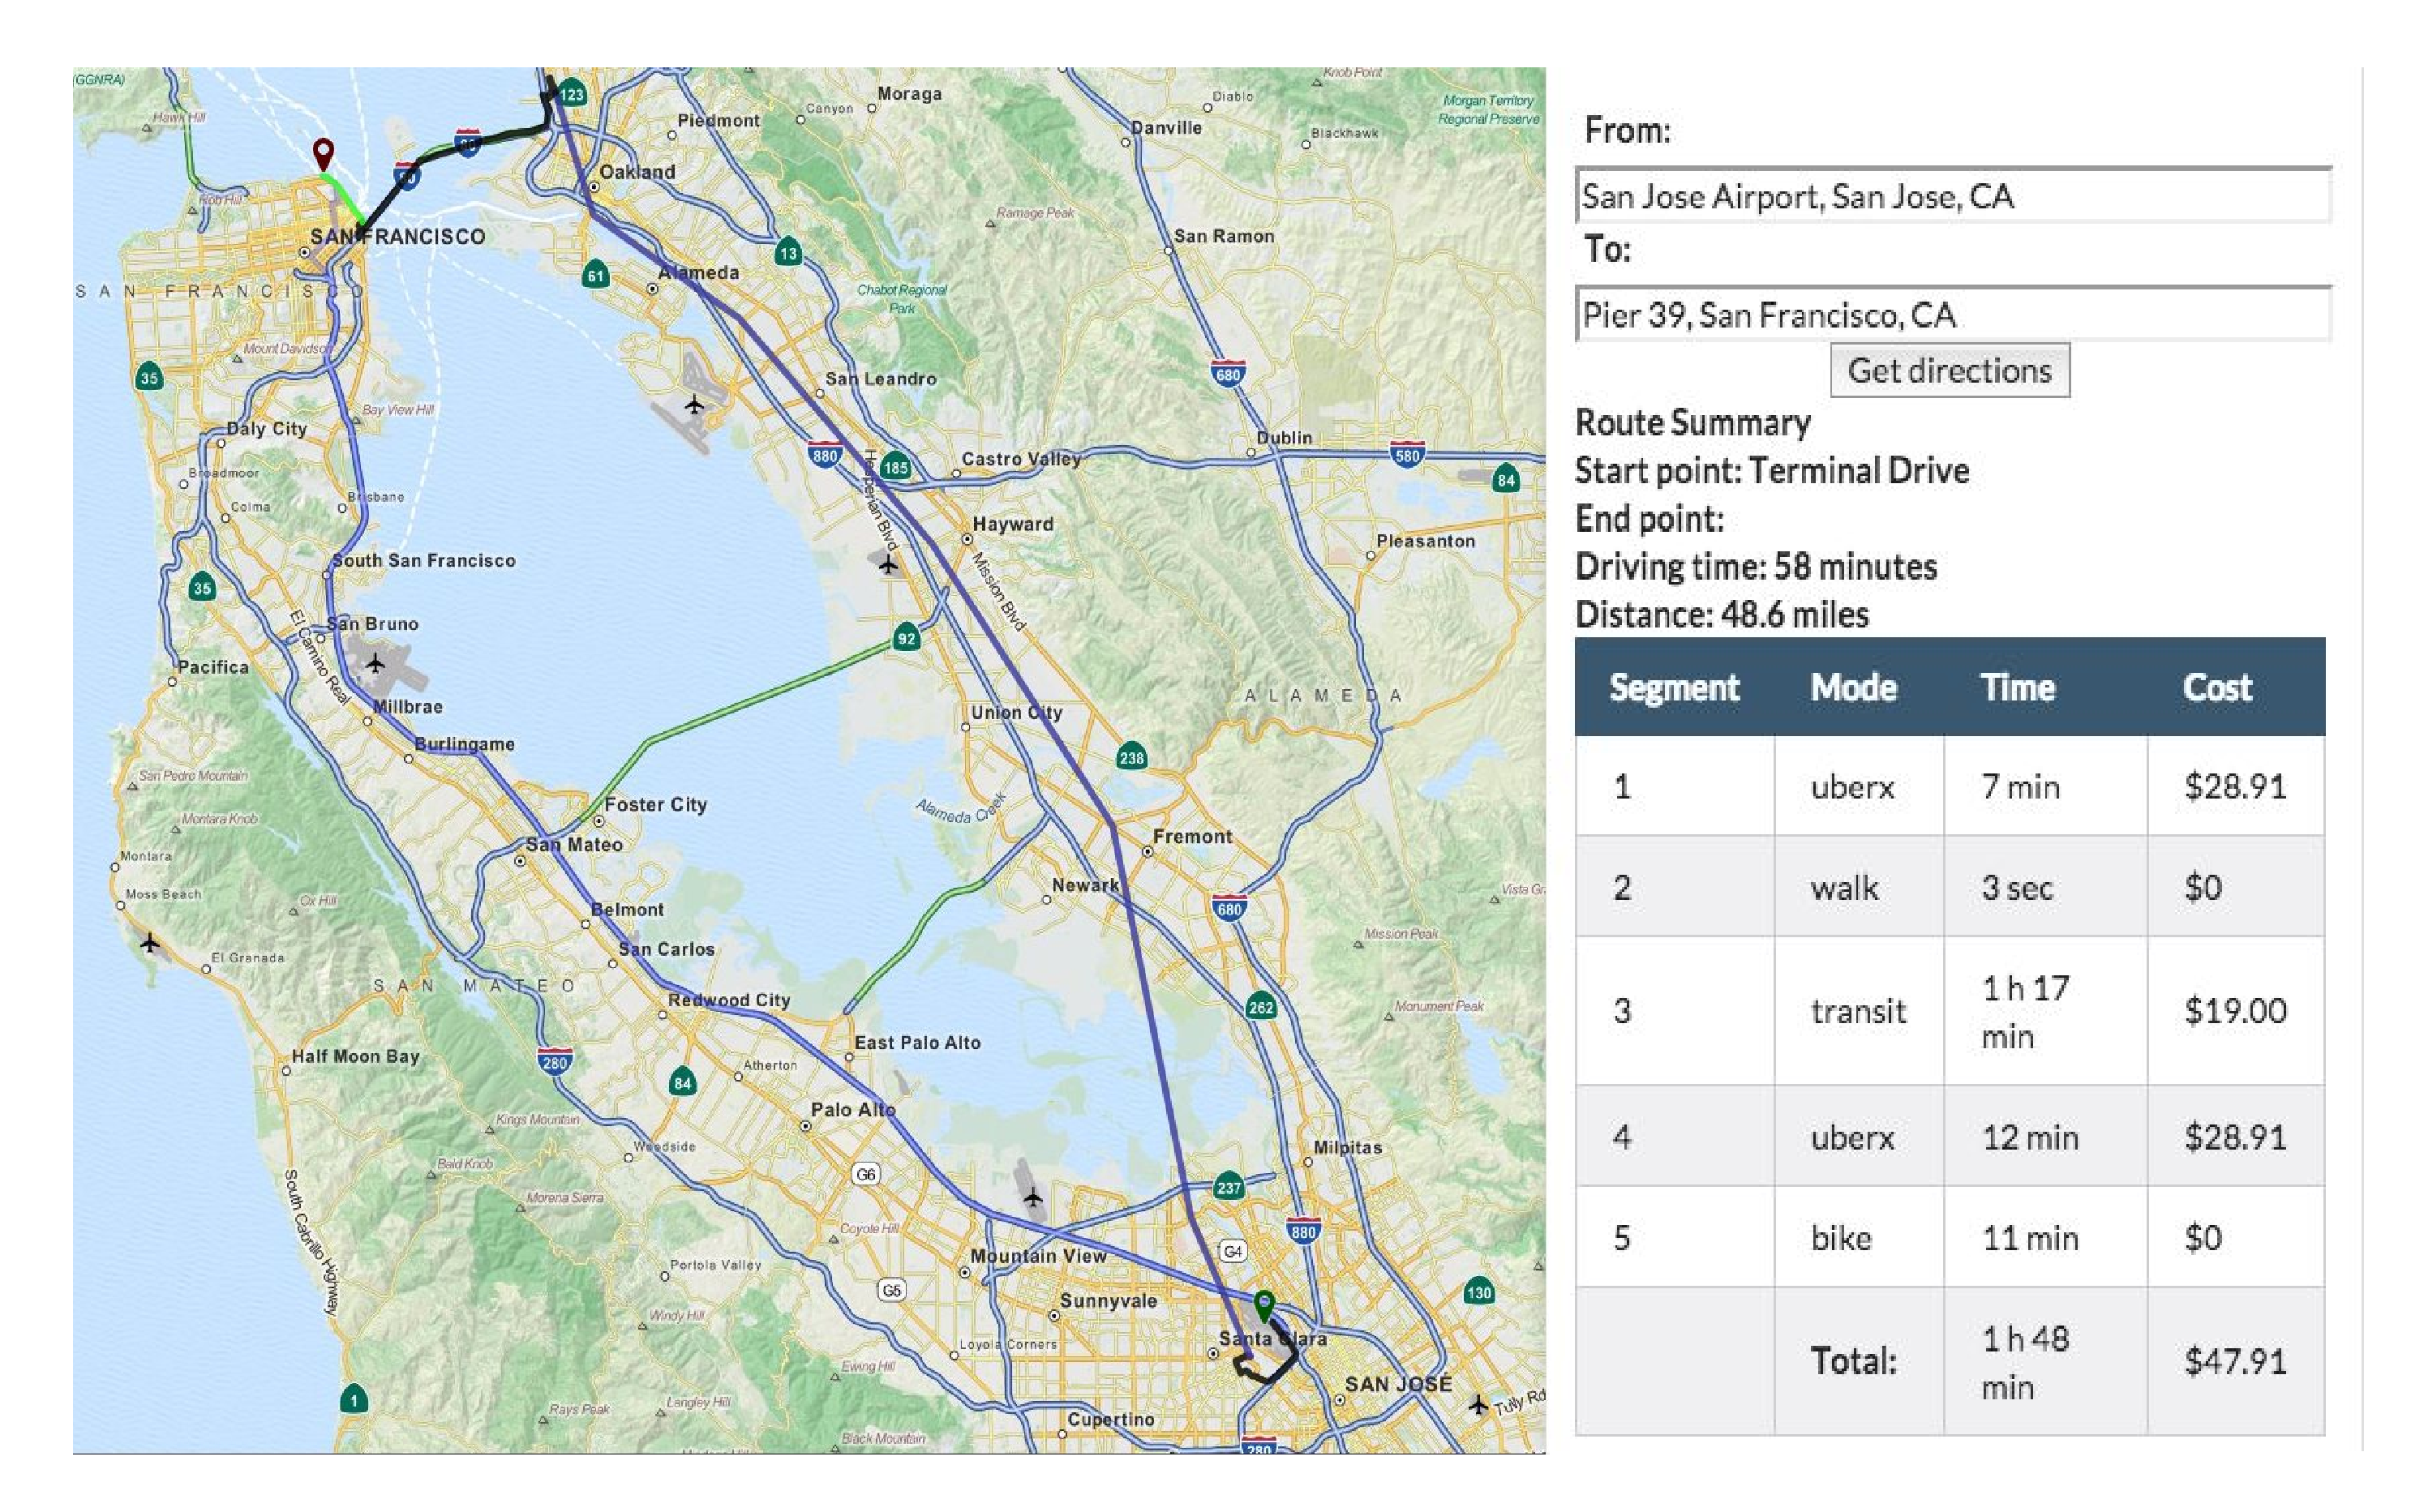
\includegraphics[width=0.5\textwidth]{figs/result_Cal.pdf}
  \caption{Resulting route for Cal\label{fig:cal}}
\end{figure}

\subsection{Auxiliary Metric}
When the user of the planner is interested in metrics other than
the ones offered already (i.e., time and fare), she might discover
new metrics (e.g., crime rates and pollution statistics), upload
them into the planner, and retrieve optimal plans taking these
metrics into account.  One scenario of this approach is the following.

Our agent needs to travel without a car across San Francisco downtown at night.
For her, safety is important.
Having found the crime statistics for the area, the agent uploads
the data as a new auxiliary metric into the map.
By specifying that she will never walk through a neighborhood
with more than fifteen crimes over the last month, and that
she would sacrifice a quarter to avoid one crime incident,
the agent tells the planner to come up with a relatively safe
route. An example is shown in \figref{crime}, where the agent
needs to start at the east of downtown and travel across the area
to arrive at the west side.  
The computed path is represented by the line colored by black,
blue and green, denoting taxi, public transit and biking, respectively.
Clearly, this path routes away from crime-heavy areas and achieves
optimality in that the combined metrics -- time, fare and crime rates,
uploaded and personalized by the user -- is minimal among all possibilities.

\begin{figure}[!ht]
  \centering
    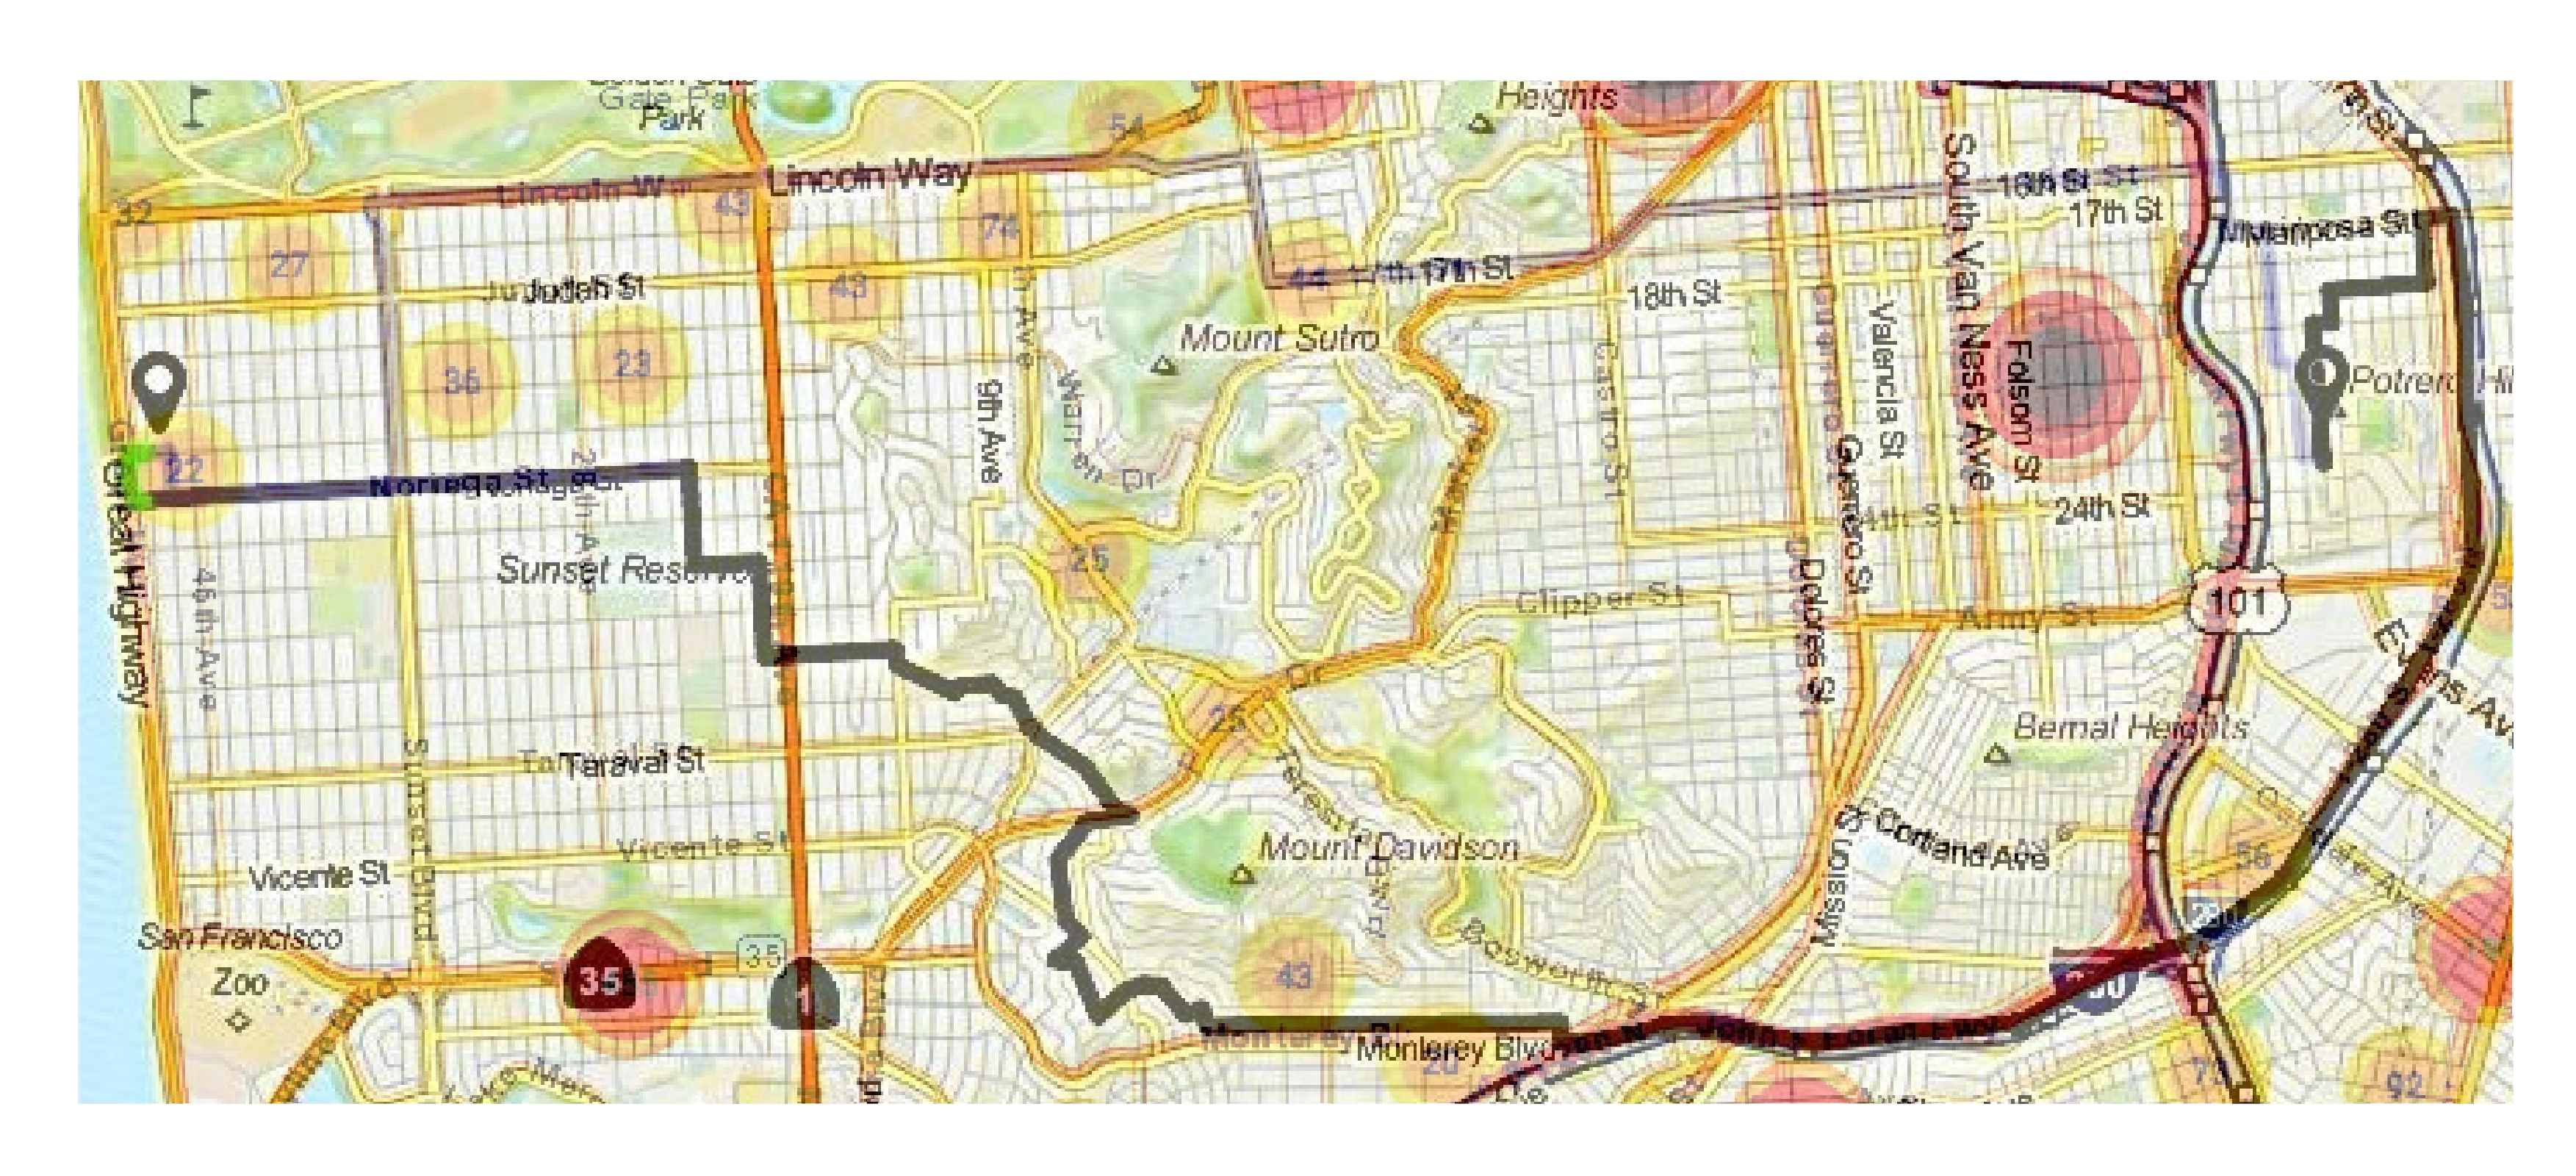
\includegraphics[width=0.5\textwidth]{figs/crime.pdf}
  \caption{Optimal route considering crime rates\label{fig:crime}}
\end{figure}
